%\addbibresource{/home/jorgsk/phdproject/bibtex/jorgsk.bib}
\subsubsection{Transcriptome sequencing with RNA-seq}
The work presented in this thesis that deals with polyadenylation is based on
sequencing data from RNA (RNA-seq) made with the Illumina GAIIX platform. Se
http://www.ncbi.nlm.nih.gov/geo/query/acc.cgi?acc=GSE30567 for detailed
information about the data was generated.

RNA-seq is a technique used to obtain a quantitative measure of the relative
frequencies of the different species of RNA present in a sample. RNA-seq was
introduced in 2008 and has been used to compare the differential expression of
genes, to discover new genes, and to discover novel isoforms of known genes by
finding new splice-sites and new 5\p and 3\p terminals
\cite{wang_rna-seq:_2009}.

Here we will go through the stages of the RNA-seq experiments that were
performed to produce the data that was analysed. We will then comment on the
stages of the experiment where biases can be introduced that affect the final
result. Finally we will discuss the matter of mapping the output of RNA-seq --
short RNA sequences called reads -- to the genome.

\subsubsection{RNA-seq and mapping: the method, errors, and biases}

\begin{itemize}
	\item The first step in the RNA-seq experiment is to isolate RNA from a cell sample.
	\item Second, the RNA is divided into an poly(A)+ and poly(A)- fraction. This is done
	by using a poly(T) primer that binds to the poly(A) tail. The RNA that bound
	the poly(T) primer is called the poly(A)+ fraction and the RNA that did not
	bind the primer is separated and called the poly(A)- fraction.
	\item Next, the RNA samples are treated to remove ribosomal RNA (rRNA). Since rRNA is
	by far the most abundant species of RNA in the cell, it will reduce the
	sensitivity for detecting lowly expressed transcripts if it is not removed.
	\item Next, the single stranded RNA is converted into double stranded complementary
	DNA (cDNA). This is required because Illumina sequencers sequence DNA and not
	RNA. To turn RNA into cDNA it is necessary to use primers -- short sequences
	that bind RNA and DNA -- that the reverse transcriptase enzyme needs for
	synthesizing cDNA on the RNA template. At this step, it is important when
	studying polyadenylation that at least some of the primers are poly(T) primers,
	otherwise the poly(A) tail will may not be converted into cDNA. Since the
	poly(T) primers can bind anywhere in the poly(A) tail, the lengths of the
	poly(A) tails will be reduced after this step.
	\item After this, the original RNA is degraded so only the double stranded cDNA
	remains.
	\item The next step is to fragment the cDNA into smaller pieces, usually by
	sound waves (sonication), to reach a desired average fragment size (usually
	around 300 nt)
	\item Finally, Illumina-patented adapters are added to the 3\p and
	5\p ends of the cDNA and the cDNA is amplified from these adapters with PCR.
	PCR amplification is necessary to get the volume of DNA required by the
	sequencing machines. Now the cDNA is ready for sequencing.
\end{itemize}

During sequencing, the double stranded cDNA is split into single strands, and
both strands are sequenced. This has the effect that sequencing outputs the
reverse-transcribed version of the original RNA molecule in addition to the
original. This is fortunate when studying polyadenylation, since as can be seen
in Figure X, it is often from the reverse-transcribed version of a transcript
that the poly(A) tail is sequenced, then in the form of a poly(T) leader. That
is, 5\p CCCGAAAA 3\p will be output as 5\p TTTTCGGG 3\p. This bias is due to
the fact that sequencing happens in the 3\p to 5\p direction, and that the read
length is shorter than the fragment length (76 bp vs 300 bp in Figure X).

It is important to note that when sequencing homopolymers like poly(A) or
poly(T) stretches, there is an increase in sequencing error rates with the
Illumina platform \cite{minoche_evaluation_2011}. This implies that when
sequencing a poly(A) sequence, other nucleotides than just A will be reported
with a relatively high probability compared to the rest of the output sequence.

\begin{figure}[htb]
	\begin{center}
		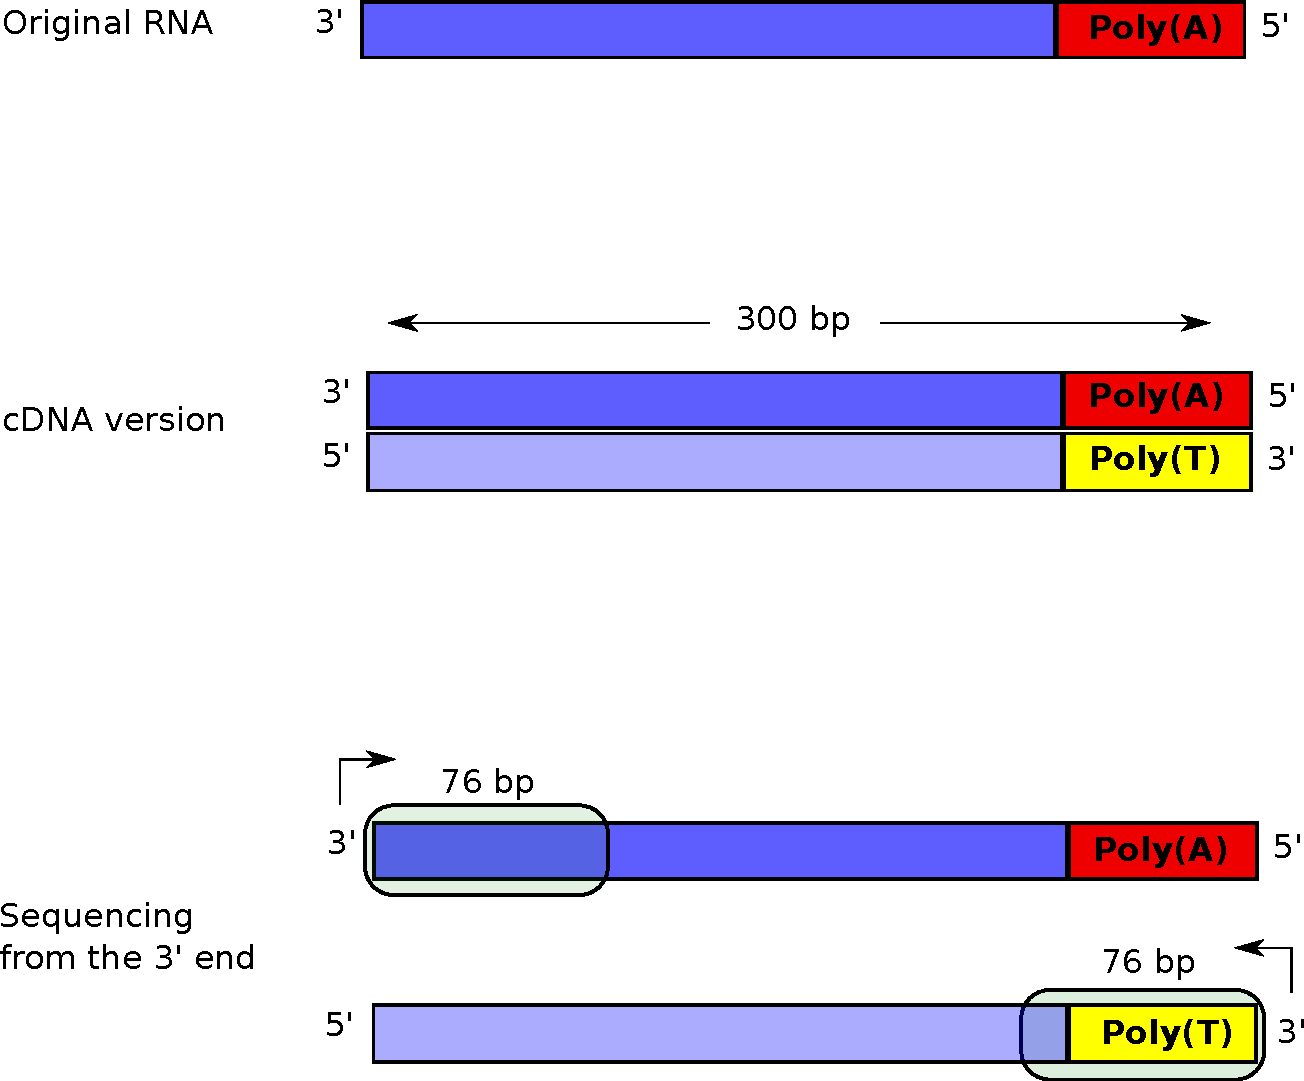
\includegraphics[scale=0.4]{figures/introduction/polyT_sequencing.pdf}
	\end{center}
	\caption{When sequencing poly(A) sites it is normally the
	reverse-transcribed version of the transcript that is actually sequenced}
	\label{fig:polyT_seq}
\end{figure}

\subsubsection{Mapping reads to the genome}
The sequence-snippets that are output from sequencing machines are called
reads, and generally come in sizes from 30 to 500 basepairs, depending on the
technology used. For the data used in this study, the read size was 76
basepairs. If a reference genome exists for the organism from which the RNA
sample was taken, these reads can be mapped to that genome to find out where
the RNA originated from. Mapping a read to the genome means trying to find
where the RNA-snippet from the sequencing machine originated from. All methods
that do this mapping allow for mismatches between the read and the genome to
allow for sequencing errors. 
